
\documentclass[apj]{emulateapj}

\usepackage{graphicx}
\usepackage{amssymb}
\usepackage{amsmath}
\usepackage{natbib}
\usepackage{color}
\bibliographystyle{apj}
\usepackage[breaklinks,colorlinks,citecolor=blue,linkcolor=magenta]{hyperref}
\shortauthors{Zhou et al.}

%%% new command %%%
\newcommand{\ima}{\texttt{ima} files }
\newcommand{\flt}{\texttt{flt} files }
\newcommand{\eps}{$\mathrm{e}^{-}/\mathrm{s}$}
\newcommand{\tinytim}{\textit{Tiny Tim}}
\newcommand{\bpic}{$\beta$ Pic}
\newcommand{\vsini}{$v\sin i$}
\newcommand{\mjup}{M$_{\mbox{Jup}}$}
\begin{document}

\title{Discovery of Rotational Modulations in the Planetary-mass
  Companion 2M1207b: A Slow Rotation Period and Cloud Height in a Low
  Gravity Atmosphere}
\shorttitle{Variability of 2M1207 b}
\author{Yifan Zhou\altaffilmark{1}, D\'aniel Apai\altaffilmark{1,2,3},
  Glenn Schneider\altaffilmark{1},  Mark S. Marley\altaffilmark{4}}

\altaffiltext{1}{Department of Astronomy/Steward Observatory, The
  University of Arizona, 933 N. Cherry Ave., Tucson, AZ, 85721, USA,
  \href{mailto:yifzhou@email.arizona.edu}{yifzhou@email.arizona.edu}
}
\altaffiltext{2}{Lunar and Planetary Laboratory, The University of
  Arizona, 1640 E. University Blvd., Tucson, AZ 85718, USA}
\altaffiltext{3}{Earths in Other Solar Systems Team, NASA Nexus for
  Exoplanet System Science}
\altaffiltext{4}{NASA Ames Research Center, Naval Air Station,
  Moffett Field,Mountain View, CA 94035, USA}

\begin{abstract}
  Rotational modulations of brown dwarfs have recently provided
  powerful constraints on the properties of ultra-cool atmospheres,
  including longitudinal and vertical cloud structures and cloud
  evolution. Furthermore, detection of periodic light curve  can directly probe the rotational periods of ultra-cool objects.

  We present here, for the first time, time-resolved high-precision
  photometric measurements of a planetary-mass companion, 2MASS1207b,
  to a brown dwarf primary. Using HST/WFC3 observation and point
  spread function fitting photometry with two spacecraft roll angles,
  we detect photometric modulations in the light curve. The amplitudes
  are 1.45\% in the F125W and 0.92\% in the F160W filters; we find a
  consistent period of $10.2^{+0.9}_{-0.8}$
  h and similar phase in both bands by fitting sinusoids to the light curves. {\color{red}The relative amplitudes in the two filters are very similar to
  that found in a recent study of a field (high-gravity) L-dwarf,
  suggesting that the cloud structures that introduce the photometric
  modulations are similar in high- and low-gravity
  objects.} Importantly, our study also measures, for the first time,
  the rotational period for directly an imaged planetary-mass companion.
\end{abstract}

\keywords{brown dwarfs -- planets and satellites: atmospheres -- planets
  and satellites: individual (2M1207 b) -- techniques: photometric}
\maketitle
%
\section{Introduction}


Presence of condensate clouds is one the most unique and essential
features of the ultra-cool atmosphere of direct imaged exoplanet and
brown dwarfs. The studies of formation and properties of condensate
clouds \citep[e.g.][]{Ackerman2001, Burrows2006a, Helling2008,
  Allard2012} have achieved great improvement in understanding the
cloud behavior across different spectral types, especially in the
explanation of L-T transition \citep[e.g.][]{Burrows2006a,
  Marley2010}.  Surface gravity is suggested to be another key
parameters in defining cloud structures besides spectral type. Low
surface gravity objects (e.g. HR8799 bcd, \cite{Marois2008a}, 2M1207
b, \cite{Chauvin2005}) show significantly redder color compared to
their spectral type matched brown dwarfs.  The anomalous colors of low
surface gravity objects are best explained by the existence of thick
clouds \citep{Barman2011, Skemer2011, Skemer2012}. However, due to
lack of observational constraint, the dependence of cloud properties
on surface gravity is not very well modeled.

Intensity modulations introduced by heterogeneous clouds can be
directly observed and studied via time resolved observation and
rotational mapping. These techniques isolate the effect of cloud
properties and obtained great success in determining the rotation
period and unveiling the structures of the atmosphere of brown dwarfs
\citep[e.g.][]{Apai2013,Buenzli2012,Buenzli2015,Burgasser2013,Radigan2012,Yang2014,Metchev2015}. \cite{Kostov2013}
demonstrated the great potential of these techniques in the study of
the cloud properties of direct imaged exoplanets and planetary mass
companions. However, high contrast magnifies
the challenges for direct imaged exoplanets and planetary mass
companions to acquire high-precision light curves comparing to brown dwarfs.

2M1207 b is a planetary mass companion that has mass of
$\sim 2.3-4.8M_{\mathrm{Jup}}$ \citep[][]{Barman2011} and an angular separation of $0.78''$ to its
host 2M1207 A, an M8 brown dwarf. Moderate contrast  \citep[6.7 mag
in J-band,][]{Mohanty2007} makes it one the most feasible
planetary mass companions for high-precision time-resolved observation.

In this {\em Letter} we present the first, high-cadence, high-precision,
time-resolved {\em Hubble Space Telescope} (HST) photometric time
series of 2M1207 b, a directly imaged planet or
planetary-mass object. We successfully detect rotational modulation
and measure the amplitudes in two bands and determine the rotational
period.

\section{Observation}

\begin{figure*}
  \centering
  \plottwo{original}{subtracted}
  \caption{WFC3 F160W images for 2M1207 system. {\em Upper panel}:
    original image, the position of 2M1207b is indicated using white
    circle.   {\em Lower panel:} residual image -- after the
    subtraction of the hybrid PSF, 2M1207 B is detected at a high significant level.}
  \label{fig:1}
\end{figure*}

We obtained direct images of the 2M1207A+b system on UT 2014 April 11
from 08:07:47 to 16:53:18 using HST and its Wide Field Camera 3
\citep[WFC3, pixel scale=$\sim0.13''$, ][]{Kimble2008} in the frame of
the HST Proposal GO-13418 (PI: D. Apai). We acquired the observations
in filters F125W ($\lambda_{\mathrm{pivot}}$ = 1245.9 nm, full width
at half maximum (FWHM) = 301.5 nm) and F160W
($\lambda_{\mathrm{pivot}}$ 1540.52, FWHM = 287.9 nm), roughly
corresponding to the J and H bands. We used the $256\times256$ pixels
sub-array mode to avoid memory dumps during the observations.  In
order to provide a near-continuous coverage for detecting modulations
we observed the 2M1207 system in 6 consecutive HST orbits, obtaining
data with cadence of $\sim1.5$ minutes over a baseline of 8 hours and
40 minutes. The observations were interrupted by 58 minutes long Earth
occultations every 94 minutes.

The observations applied space craft rolls between each two orbits to
allow roll-subtraction of the primary \citep[e.g.][]{Song2006}. The
telescope roll angles for orbit 1, 3, and 5, and those for 2, 4, and
6 differ by $25^{\circ}$. At the separation of 2M1207 b, this angle
difference corresponds to a displacement of $0.34''$, or 2.75 and 2.30
resolution elements in F125W and F160W, respectively. In each orbit we
took 8 SPARS10 exposure sequence with NSAMP=10,
alternating between F160W and F125W filters, with 2--3 identical
exposures in one exposure sequence. To improve sampling and reduce the
risk that point spread function (PSF) lays on bad pixels, we applied a
4-point dither pattern with differential "X/Y" offsets of 1.375" in
the detector frame, providing optimal non-integral (half pixel)
stepping of 10.5 and 8.5 pixels in F125W and F160W, respectively. Over
the 6 orbits, we obtained 70 images with 10 non-destructive read-outs
in F125W and 64 images in F160W with exposure time of 88.4~s for both
filters.

\section{Data Reduction}

 \begin{figure*}
  \centering
  \plotone{systematics}
  \caption{F125W (left) and F160W (right) light curves under different
    variability verification tests. Individual measurements are
    plotted with gray crosses. Photometric measurements of the same exposure
    sequence are binned, and binned photometry are plotted with points
    or squares. Best fitted sinusoidal curves are plotted with solid
    lines. {\em Upper}: binned measurements taken in dithering
    position 1 and 3 (red points) and that taken in 2 and 4 (blue
    squares) are plotted with different symbols. They demonstrate same
    trend of modulation. In upper left panel, green line is sinusoidal
    wave fitted with all parameter set free, and purple line is
    sinusoidal wave fitted with period set the same as that of
    F125W. {\em Middle}: sinusoidal waves fitted without using the
    data taken in Orbit \#1. These curves are almost identical to the
    curves plotted in upper panel. {\em Lower}: photometry measured
    with AFEM-added images and best fitted sinul curves. These
    points and curves are also almost identical to those plotted
    in the upper panel.}
  \label{fig:2}
\end{figure*}

\subsection{Photometry}

We start the reduction from the \flt{} produced by the WFC3's
\texttt{calwfc3} pipeline. We do not opt to use \ima{} that contain
all non-destructive read-outs, because these provided less information
on 2M1207A, which saturated after the first few samples.  The \flt{}
are results of basic calibration, including dark current correction,
non-linearity correction, flat field correction, as well as
up-the-ramp fit on the non-destructive read-outs. From the beginning,
pixels with data quality flags ``bad detector pixels'', ``unstable
response'', and ``bad or uncertain flat value'' are masked out and
excluded from further analysis as suggested by previous transit
exoplanet spectroscopic observations\citep[e.g.][]{Berta2012,
  Kreidberg2014}.


One major challenge of high contrast imaging observation using WFC3/IR
is significant under-sampling of the detector.  2M1207 A and b are
only separated by $\sim6$ pixels or $\sim$5 FWHM of the PSF. When
applying roll subtraction, notable artifacts are generated
by image shifting and interpolation. On the other hand, \tinytim{} PSF
simulator\citep{Krist1995} offers a solution by providing Nyquist or better
sampled PSF, but systematic errors of \tinytim{} PSF for WFC3 limits
its ability in high precision photometry\citep{Biretta2014}. However,
we are able to fully characterize the difference of model and observed
PSFs with 6 orbits time-resolved observation data. To obtain robust \tinytim{} PSF
photometry, we design a 2-round PSF fitting strategy: 1. calculating
correction map for \tinytim{}; 2. hybrid PSF photometry.

For both of 2 rounds, we use \tinytim{} to calculate 10$\times$
over-sampled model PSFs based on the filters, the spectra
\citep{Bonnefoy2014, Patience2010}, the telescope's actual focus, and
the telescope jitter.  We use the set of \tinytim{} parameters
provided by \cite{Biretta2014} to improve modeling  the cold mask, OTA
spikes, and the coma. The focus parameters are calculated using the
model listed on the STScI
website\footnote{\url{http://www.stsci.edu/hst/observatory/focus/FocusModel}}.
To register the \tinytim{} PSF to the observed PSF of 2M1207 A, we move the
over-sampled PSF on a coordinate grid (gird size=0.001 pixel) using
cubic interpolation, and search for the position that minimizes the
rms difference of the observed and re-binned \tinytim{} PSFs over a
region centered on 2M1207 A with a 5-pixel-radius aperture centered on
2M1207 b excluded.  Then we introduce another \tinytim{} PSF for
2M1207 b and fit the position of 2M1207 b and the scales of the
/tinytim{} PSFs of 
2M1207 A and b simultaneously with least square optimization. From the
first round fit, we discover that the difference of observed PSFs and model
PSFs are very stable for given PSF positions. Therefore, at the end
of the first round PSF fitting, we derive 8 (2 roll angles $\times$ 4
dithering positions)  correction maps for each
filter:
\begin{equation}
  \mathrm{Corr = Median(PSF_{obs.} - PSF_{model} )}
\end{equation}
where $\mathrm{PSF_{model}}$ is a combination of two \tinytim{} PSFs
for 2M1207 A and b. In the second round, we combine the correction
term linearly with the two \tinytim{} PSFs to generate hybrid PSFs,
and fit the three components together. We find that by introducing the correction term,
the reduced $\chi^{2}$ of PSF fitting is decreased from $\sim 10$ to
$\sim 1$. Relative photometry is acquired from the scaling
parameters of the \tinytim{} PSFs.

PSF profiles change with exposure positions due to
pixelation, especially for the case that WFC3 IR is significantly
under-sampled. Also, the flat fields may potentially have large scale
structures \citep{dressel2012wide}. We find a correlation of
photometry with PSF positions on detector frame for both 2M1207 A and
b. Correction is made by normalizing each group of
exposures that have the same dithering position and telescope roll angle
individually -- we take the median of the fluxes that are measured
from these exposures as normalization factors and divided them from
every photometric measurement. Because the normalization factor for
each group of exposures is calculated across the whole observation in
time domain,
this step has negligible impacts on variability
analysis.

  \begin{figure*}
  \centering
  \plotone{sineCurveFit_binCombined}
  \caption{Normalized light curves for 2M1207 B (upper) and A (lower)
    with filter F125W (left) and F160W (right). Individual photometric
  measurement are plotted in gray crosses and binned photometry are
  plotted with red points. Best fitted sinusoidal waves are plotted
  with blue solid lines.}
  \label{fig:3}
\end{figure*}



\subsection{Uncertainty Analysis: White noise}

First we estimated the photon noises for the photometry of
2M1207b. The total photon noise of the photometry is calculated by
combining the photon noise of every single pixel that is calculated
from count rates and detector gain. The photon noises for photometry
in F125W and F160W are 1.33\% and 1.02\%, respectively.

Since the PSFs for the 2M1207 A and b are fitted simultaneously, the
uncertainties of photometry and position for the primary and secondary
are coupled. Imperfection of position measurement of 2M1207 A could
potentially significantly affects the photometry of 2M1207 b. We used a Monte Carlo
(MC) method to evaluate the overall systematic of the PSF fitting. We
applied the PSF photometry to images that were added with random
Poisson noises and repeat the photometry procedure for 1000
times. From the distribution of the result, the uncertainties for F125W
and F160W photometry are 1.34\% and 1.12\%, respectively. We conclude
that the white noise of our observation is dominated by photon noise.

\subsection{Uncertainty Analysis: Flat field uncertainties}


2M1207 b were observed at 8 different spots on the
detector (2 rolls $\times$ 4 dithering positions). Imperfect flat
field correction can potentially introduce position-dependent differences in the count rates. The
uncertainty of WFC3 IR pipeline flat field is typically $\sim 1\%$
\citep{dressel2012wide}.

In PSF photometry, however, multiple pixels are fitted simultaneously
and we expect to be less affected by high spatial frequency flat field
noise, and a lower than 1\% uncertainty from the flat field
errors. To verify this, we multiplied every image by an artificial flat
field error mask (AFEM) -- a uniformly distributed Gaussian noise array with
mean of 1 and sigma of 1\% -- and repeated the PSF photometry on the
resulting images.  The analysis of these experiments showed almost
identical light curve to the original, verifying that the flat field
errors do not affect our photometry significantly (Figure
\ref{fig:2}, bottom panel).


\section{Verification of Photometric Modulations and Amplitude
  Estimate}

\begin{figure*}
  \centering
  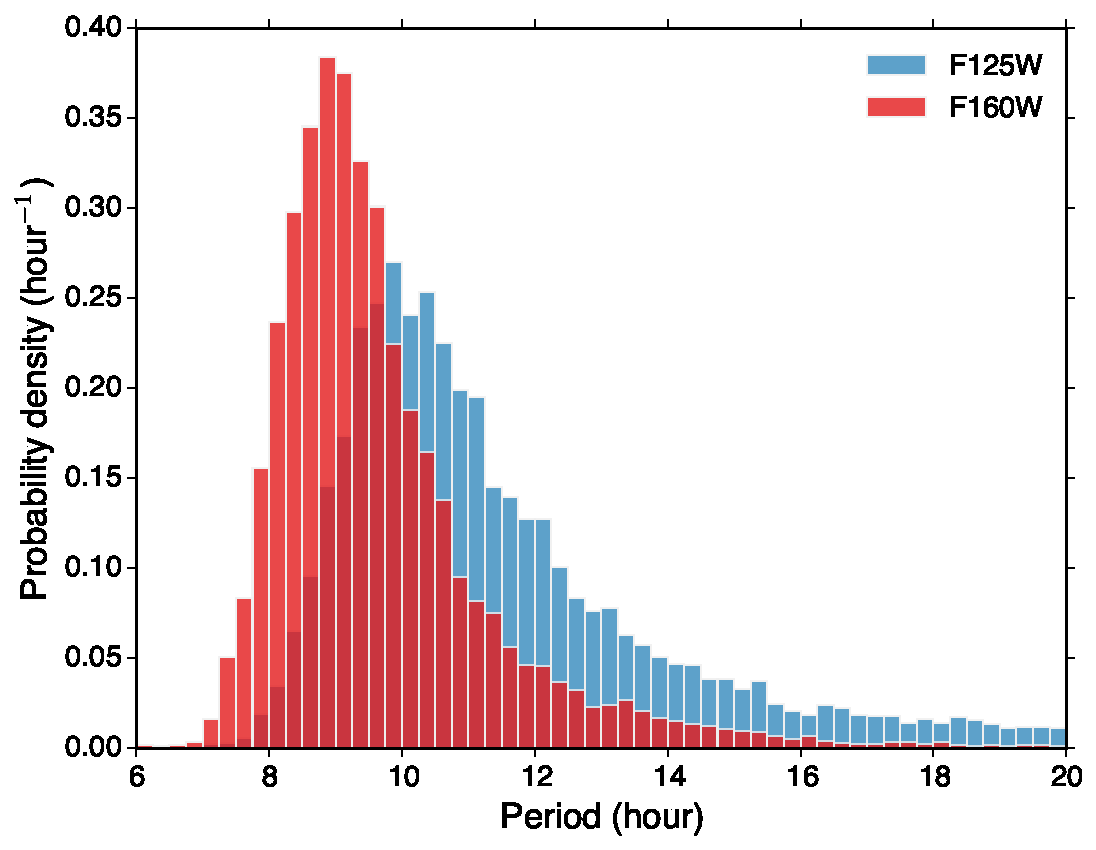
\includegraphics[width=0.45\textwidth]{periodDistr}
  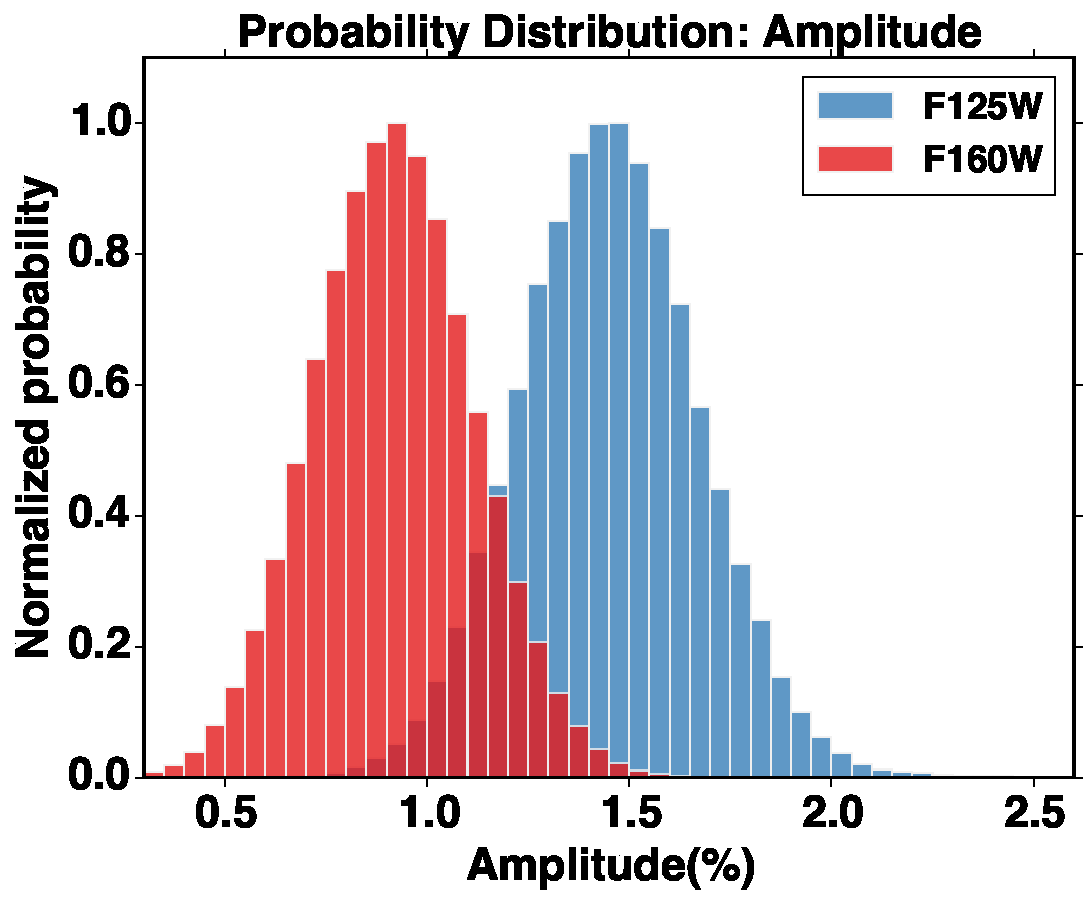
\includegraphics[width=0.45\textwidth]{amplitudeDistr}
  \caption{Distributions for periods (left) and amplitudes(right) for the light
    curve of F125W and F160W. The bin size for histograms of period is
  0.25 hour and for that of amplitude is 0.5\%. Histograms are
  normalized in the way that total area of the histogram equals to
  1. In the right panel, Gaussian profiles are fitted to the
  histograms of periods and plotted in solid lines.}
  \label{fig:4}
\end{figure*}

\subsection{Tests and Verification}

The light curves that result from our photometry show apparently
sinusoidal modulations, discussed in more details in
\S,\ref{Results}. To verify that these modulations are intrinsic to
the object and not results of our data reduction procedures or due to
instrumental changes, we carry out three different tests.

First, we fit sinusoids independently to the light curves of two filters to verify
the similarity of the signal in the two bands (Figure \ref{fig:2}, top
panel). Inconsistent periods or
light curve shapes would argue against a genuine signal.  We find
that the periods of the best fit sine waves are similar,
$10.5^{+1.2}_{-1.3}$h for F125W and $9.1^{+1.1}_{-1.0}$h for
F160W. These periods are roughly consistent within the
uncertainty. Furthermore, these periods are not close to any
timescales over which HST or WFC3 are known to changes.

As a second test, we repeat the analysis neglecting the first
orbit. The motivation behind this test is that, due to spacecraft
thermal settling, the first orbits of HST observations are often
slightly unstable, and neglected in high-precision studies
\citep[e.g.][]{Mandell2013}. Indeed, in our analysis 2M1207 A is
significantly fainter in the first orbit (Figure \ref{fig:3}) than in
the subsequent ones.  Our analysis based on orbits 2--6 finds
essentially identical results to our analysis using the whole 6 orbits, based on
which we conclude that the first less reliable orbit does not affect
our results significantly (Figure \ref{fig:2}, middle panel).

As a third test, we explore whether a subset of images, perhaps due to
imperfectly normalized or correlated with specific instrument states,
can drive the light curves into an apparently sinusoidal shape. To
test this possibility, we split the data into two temporally
overlapping halves: subset one are images taken at dithering position
1 and 3, and subset two are those taken at dithering position 2 and
4. For both data-sets, we repeated our analysis independently.  For
both of F125W and F160W, two halves demonstrated similar trend of
variability.  Our analysis detect sinusoidal modulations in {\em
  both} subsets and in {\em both} filters, with periods and
amplitudes consistent with those derived from the complete data set
(Figure \ref{fig:2}, upper panel).
 
 These tests demonstrate that the modulation seen in our data are
 consistently present in the different filters, in the different time
 segments of the data, and in data obtained in different dithering
 positions. All of the three tests support the modulation signal to be
 intrinsic to the target. 
 

\subsection{Amplitude and Period Measurements}

We use a MC method to analyze the light curve, and provide amplitudes
and periods as well as their uncertainties for both filters. We
generate series of random Gaussian noises with the standard deviation
same as the photon noises, add them to the original light curves, and
fit sinusoids to the newly combined light curves. We repeat above
routine for 100,000 times and obtain the distribution of the fitting
parameters (Figure \ref{fig:4}).


\section{Result}
\label{Results}

We present the first high-resolution, high-cadence, and high-precision
photometry of a directly imaged planet or planetary-mass
companion. Our observations reveal a modulation in the light curve of
the $\sim 4 \mathrm{M_{{Jup}}}$ companion 2M1207b, the first detection
of modulations in directly imaged planetary mass objects.  The best
fitted periods for F125W and F160W are 10.5 and 9.1 hour,
respectively. The modulation amplitudes for the normalized light
curves are 1.45\% and 0.92\% for F125W and F160W light curves.

We obtain high signal to noise photometry series for both 2M1207 A
and B (Figure \ref{fig:3}). On average, the photometric contrast is
$6.52\pm0.01$ mag for F125W and $5.77\pm0.01$ mag for F160W. The
difference of F125W contrast from that measured in J-band
\citep{Mohanty2007} and F160W contrast from that measured with NICMOS
F160W \citep{Song2006} is due to the different throughput profiles of
the filters.


The distributions for the periods demonstrate long tail shaped towards
long period, with core region roughly Gaussian. With 64\% confidence,
we estimate the 1-$\sigma$ range for the periods of F125W and F160W
to be $10.5_{-1.2}^{+1.3}$ and $9.1_{-1.0}^{+1.1}$ h,
respectively. The period of best fitted sinusoid for F125W light curve
is 1.5h longer than that for F160W, which is $\sim 20\%$ larger than
1-$\sigma$. We also jointly fit the two band light curves forcing the
periods of two sinusoids to be the same. We derive a modulation period of $10.2^{+0.9}_{-0.8}$ h.

We discover that the modulation amplitudes in the two bands are significantly
different. By fitting Gaussians to the MC fit result distributions, we
determine that modulation amplitude of F125W is 1.45\% with a
standard deviation of 0.22\%, and that of F160W is 0.92\% with a
standard deviation of 0.20\%. The peaks of the two
histograms separate by more than 2-$\sigma$. The modulation amplitude
for F125W is 1.58 times of that for F160W light curve.


\section{Discussion}

\begin{figure*}
  \centering
  \plottwo{rotationDiagram}{JH}
  \caption{comparison of 2M1207's rotation period and color change
    with brown dwarfs, \bpic{} b, and solar system planets. {\em
      Left}: period vs. mass plot for 2M1207 b (red square), solar
    system planets and \bpic{} b (blue squares), and brown dwarfs
    (black circles, gray shade). The mass of brown dwarfs are assumed
    to be 30 \mjup{}. The gray rectangle that has a $\pm$15 \mjup
    range in $x$, and a $\pm \sigma$ of brown dwarf periods range in
    $y$, indicates a region where brown dwarfs most likely to appear
    in this diagram. Rotation period monotonically decreases with the
    increase of mass. {\em Right}: ratio of modulation amplitude in J
    and H band vs. spectral type for 2M1207b and brown dwarfs. The
    point for 2M1207 b is shifted to +$x$ for half spectral type for
    clarification.  The colors of the points represent J$-$H
    magnitude, and the sizes of the points are proportional to the
    J-band modulation amplitudes. The gray dashed line is the result
    of a linear fit to these points. Tight correlation of J- and
    H-band modulation amplitude ratio and spectral type is shown.}
 \label{fig:5}
\end{figure*}

% A fundamental result of our study is the direct determination of the
% rotation period of a directly imaged planetary-mass object. We
% convert the rotation period to equatorial velocity  by adopting a radius of 1 -- 1.4
% $R_{\mathrm{Jup}}$ for 2M1207b, and 1 $R_{\mathrm{Jup}}$ for field
% brown dwarfs with well defined rotation period from the study of
% \cite{Metchev2015}, and compare their rotation velocities with solar
% system planets and \bpic{} b in the left
% panel of Figure \ref{fig:5}.  The study by
% \citep[][]{Snellen2014} succeeded in measuring \vsini{} for \bpic{} b
% and demonstrated that it fits a trend defined by Solar System planets
% in which more massive planets have faster rotation rates. They suggested
% that this relation is linked to the accretion processes during planet
% formation.

A fundamental result of our study is the direct determination of the
rotation period of a directly imaged planetary mass object. In the
left panel of Figure~\ref{fig:5} we compare the rotation period of
2M1207 b to the solar system planets, \bpic{} b the only other directly
imaged planet with an estimated period and measured \vsini, and
field brown dwarfs from the study of \citep[][]{Metchev2015}.  The
study by \citep[][]{Snellen2014} succeeded in measuring \vsini{} 
for \bpic{} b and demonstrated that it fits a trend defined by Solar
System planets in which more massive planets have faster rotation
rates. The interesting finding that \bpic{} b, an exoplanet that formed
in a protoplanetary disk, follows this trend suggests a possibly
connection between planet mass, initial angular momentum, and
formation in a disk.

Excitingly, our measurement of the rotation period of 2M1207b, a
planet mass companion that has similar age to \bpic b, has a rotation
period that fits in the same trend, as well as majority of brown
dwarfs.  We note that 2M1207 b is most likely formed in the same way
as brown dwarfs by gravitational fragmentation. The result that
objects formed in different scenarios share the same trend of period
vs. mass suggests that rotation periods -- in absence of
well-determined ages -- are not good tracers of the formation pathways
and may not contribute important evidence for a formation in a disk
vs. in a cloud core environment.
%{\em Add younger BDs and this may change}
% Excitingly, our measurement of the rotation period demonstrates that
% 2M1207b, a planetary mass companion  with similar age to \bpic{} b, has a rotation velocity
% that fits in the same trend, as well as majority of brown
% dwarfs. We note that 2M1207b is most likely formed in the same way as brown
% dwarfs by gravitational fragmentation, which suggests
% that rotation periods are not good tracers of the formation pathways
% and may not contribute important evidence for a formation in a disk
% vs. in a cloud core environment.

Furthermore, our observations allow us to compare the relative
amplitudes in the J- and H-bands with the handful of brown dwarfs
for which high-quality near-infrared time-resolved observations have
been obtained. In the right panel of Figure \ref{fig:5}, we compare the
relative amplitude of J- and H-bands of 2M1207b and brown dwarfs
\citep{Apai2013,Buenzli2012,Buenzli2015,Burgasser2013,Radigan2012,Yang2014} that
have different spectral types and J$-$H colors.

We find a tight correlation between the spectral type of the object
and the J- to H-band modulation amplitude ratio. In the right panel of
Figure \ref{fig:5}, we demonstrate that earlier spectral type objects,
independent of their surface gravity, have larger amplitudes at
shorter wavelength than at longer wavelengths. Importantly, although
the J$-$H color of 2M1207b is significantly redder, its relative
modulation amplitude ratio is almost identical to the matching
spectral type mid-L dwarf 2M1821.

{\color{red}This trend can be qualitatively explained using the toy model proposed
in \cite{Yang2014} within the spectral type range of mid-L to L-T
transition. Assuming that intensity modulations are introduced by a
refractory cloud whose upper layer locates at altitude $z$, the
variation amplitude ratio for J and H band can be expressed as
$\mathrm{Amp_{J}}/\mathrm{Amp_{H}} =
\exp\left[-(\tau_{\mathrm{J}}(z)/\tau_{{\mathrm{H}}}(z)\right]$,
where $\tau_{\mathrm{J}}(z)$ and $\tau_{\mathrm{H}}(z)$ are the
optical depths of upper cloud layer for J and H bands. The opacity for
J band is smaller than that for H, therefore from mid-L to L-T
transition, as the cloud upper boundary appears higher in the
atmosphere, the optical depth difference for the two bands gets
smaller, and the amplitude ratio decreases.  We note, that the late T
dwarf 2M2228 falls exactly on this trend, but whose variations are
likely to emerge from a different mechanism as their silicate clouds
are below the visible photosphere \citep[e.g.][]{Stephens2009}.

We infer that the upper cloud layer of 2M1207b is at a similar optical
depth as that of a matching spectral type field brown dwarf from the fact
that they share similar J- and H-bands light curve amplitude ratio.
The
two processes that atmosphere opacity at certain pressure level
enhances and the cloud thickness increases with the decrease of surface
gravity have to counterbalance with each other to maintain the optical
depth of the cloud upper layer.}

\section{Conclusions}
In summary, from our J- and H-band high precision, high-cadence light
curves we discovered sinusoidal modulations in the planetary mass
object 2M1207b. This is the first detection of rotational modulations
in a directly imaged planetary mass object.  The period is
$10.2^{+0.9}_{-0.8}$, similar to that derived from \vsini{} 
measurements for the direct imaged exoplanet \bpic{} b and
significantly longer than most field brown dwarfs with known rotation
periods. The modulation amplitude ratio of J and H band is almost
identical to one matching spectral type L5 dwarf, although they have
very different J$-$H colors.

Finally, we note that the observations presented here open an exciting
new window on directly imaged exoplanets and planetary-mass
companions. Our study demonstrates a successful application of
high-cadence, high-precision, high-contrast photometry with planetary
mass companion. We also show that these observations can be carried
out simultaneously at multiple wavelengths, allowing us to prove
multiple pressure levels. With observation of a larger sample and at
multiple wavelengths, we will be able to explore the detailed
structures of atmospheres of directly imaged exoplanets, and identify
the key parameters that determine these.


\bibliography{ref.bib}
\end{document}

%%% Local Variables:
%%% mode: latex
%%% TeX-master: t
%%% End:
